\chapter{Detección de árboles basada en estratos}
\label{chap:Deteccion}
Este capítulo se dedicará a explicar el algoritmo planteado para la detección de árboles en Nubes de Puntos. La figura \ref{fig:diagFlujoAlgoritmo} representa el diagrama de flujo del algoritmo empleado para la detección de árboles, cada fase de este tendrá una sección dedicada a él explicando a fondo su funcionamiento.

\section{Estructura del Algoritmo}
\label{sec:EstrucuturaProp}

\begin{figure}[h]
\centering
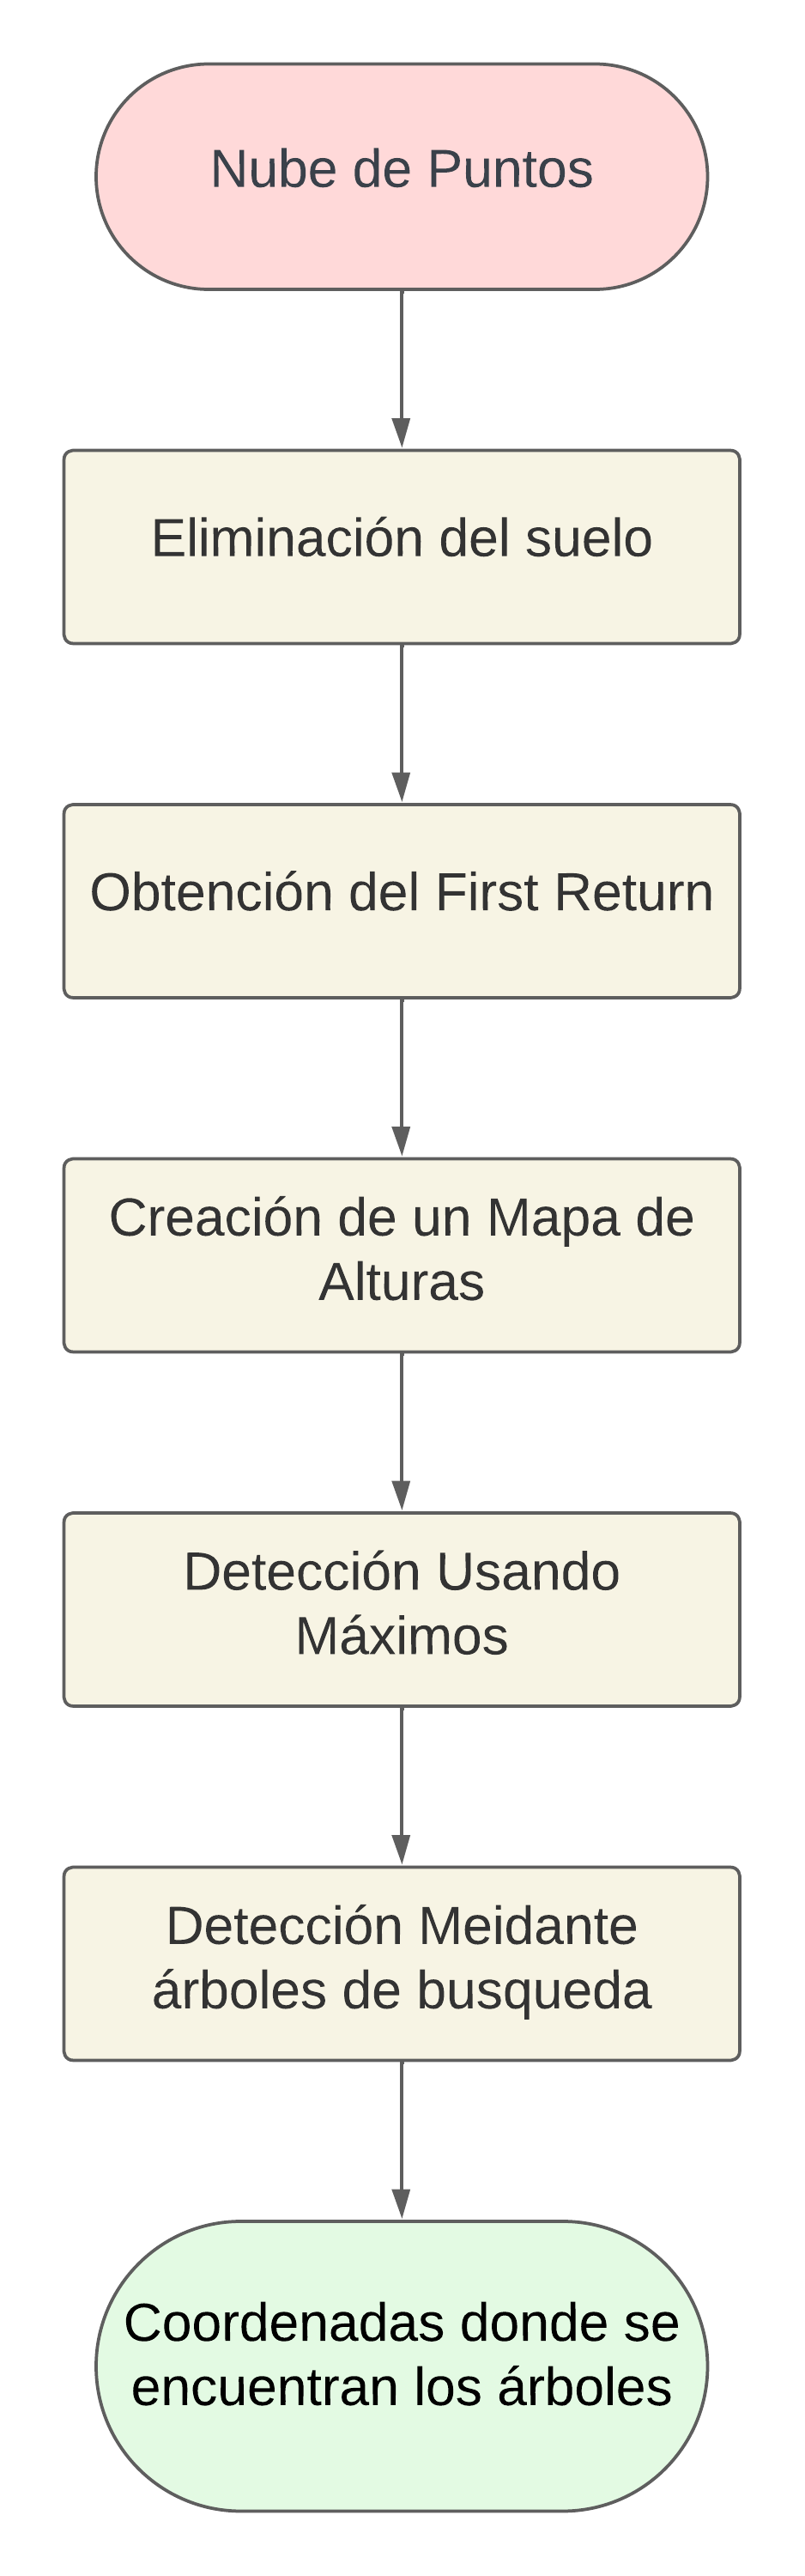
\includegraphics[height=8.5cm]{imaxes/Diagrama_alg.png}
\caption{Diagrama de Flujo del Algoritmo}
\label{fig:diagFlujoAlgoritmo}
\end{figure}


\subsection{Obtención de las Alturas Normalizadas}
\label{chap:normalAlgo}

La obtención de las alturas normalizadas, también conocidas como alturas sobre el suelo (HAG), es un paso esencial para la detección y análisis de objetos elevados, como árboles, en nubes de puntos. Las alturas normalizadas eliminan la elevación del terreno y se centran en la altura relativa de los objetos con respecto a la superficie del suelo.
Esto nos ayuda a reducir errores provocados por los diferentes desniveles del terreno y nos ayuda a la comparación de los resultados entre diferentes regiones ya que nos concentramos únicamente en la verticalidad de los puntos que conforman los arboles.

\begin{figure}[h]
  \begin{subfigure}{0.5\textwidth}
    \centering
    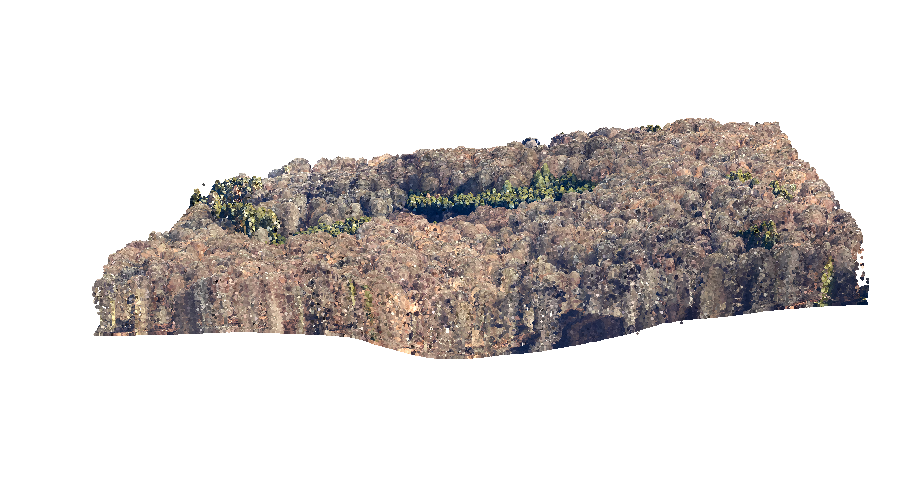
\includegraphics[width=0.8\linewidth]{imaxes/nohag.png}
    \caption{Nube de puntos sin alturas normalizadas}
    \label{fig:sub1}
  \end{subfigure}%
  \begin{subfigure}{0.5\textwidth}
    \centering
    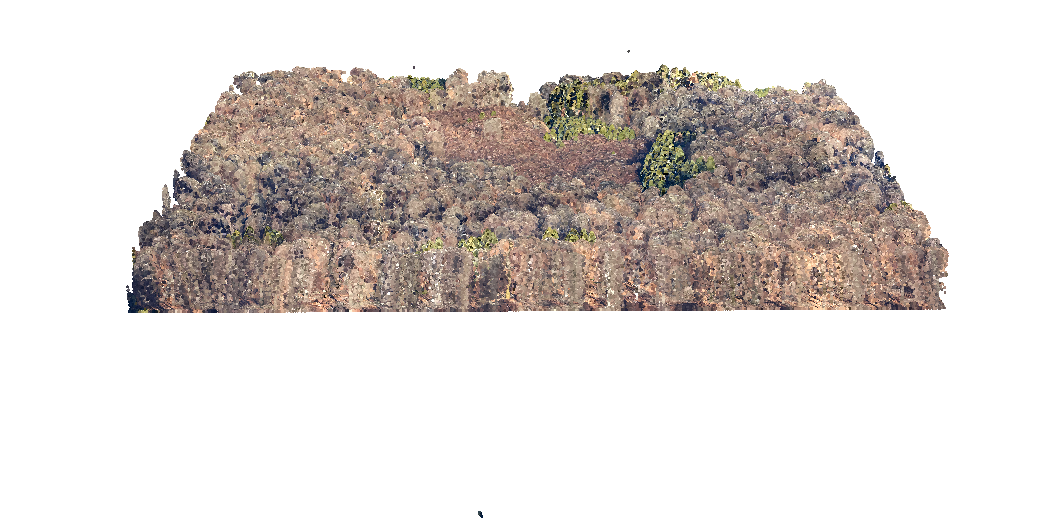
\includegraphics[width=0.8\linewidth]{imaxes/hag.png}
    \caption{Nube de puntos con alturas normalizadas}
    \label{fig:sub2}
  \end{subfigure}
  \label{fig:algo1}
\end{figure}

\subsection{Obtención del Last Return}
\label{chap:LastAlgo}

Esta parte es fundamental en este algoritmo. El uso del último retorno en la detección de árboles mejora la visualización y la caracterización del tronco, debido a que este retorno sufre menos interferencia de la vegetación y ruido. Al alcanzar la cima del árbol, proporciona una visión directa del tronco sin obstrucciones de las hojas y ramas superiores. Esto permite una identificación más precisa de la altura, forma y detalles del tronco, siendo esencial en aplicaciones como análisis de vegetación y modelado del entorno.

\subsection{Eliminación del suelo}
\label{chap:groundAlgo}
En esta primera fase, el objetivo es eliminar los puntos que corresponden al suelo, ya que no son necesarios para la detección y su inclusión solo requeriría un mayor consumo de recursos. Para este paso, se utilizó el algoritmo basado en simulación de ropa de Zhang, el cual está disponible en PDAL.

El método CSF crea una malla virtual que abarca toda la nube de puntos y luego ajusta dicha malla a los puntos de la nube. A cada punto se le estima la altura de la malla mediante la interpolación de los puntos dentro de cada triángulo. Luego, se identifican los puntos que constituyen ruido al comparar la altitud de los puntos de la nube con la altitud estimada en la malla.

Esta aproximación nos permite filtrar los datos de manera sencilla, sin requerir una gran cantidad de parámetros, y proporciona resultados precisos.

\begin{figure}
  \begin{subfigure}{0.5\textwidth}
    \centering
    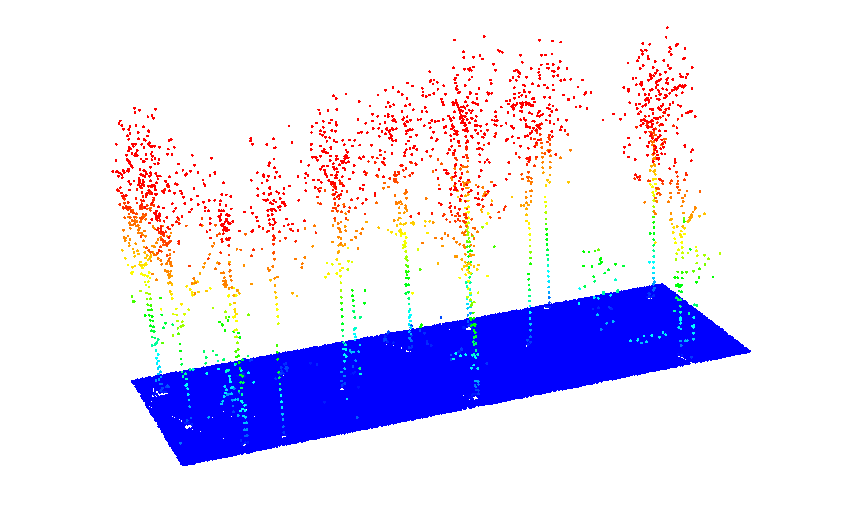
\includegraphics[width=0.8\linewidth]{imaxes/last.png}
    \caption{Nube de puntos con los últimos retornos}
    \label{fig:last1}
  \end{subfigure}%
  \begin{subfigure}{0.5\textwidth}
    \centering
    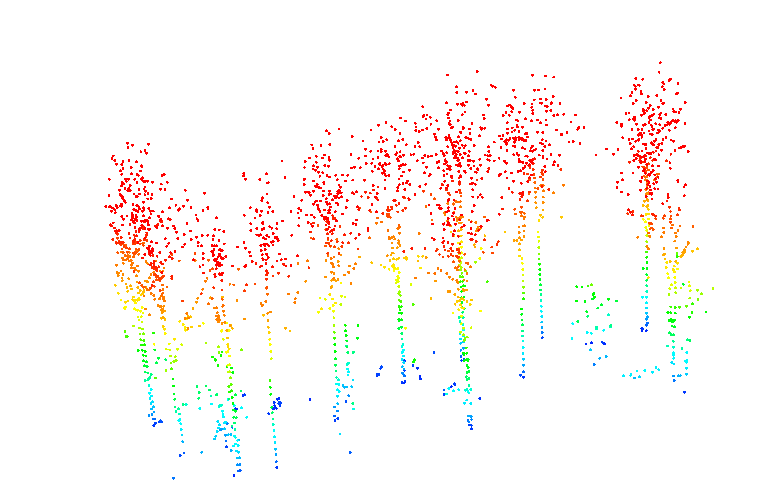
\includegraphics[width=0.8\linewidth]{imaxes/lastnog.png}
    \caption{Nube de puntos con últimos retornos sin suelo}
    \label{fig:last}
  \end{subfigure}
  \label{fig:algo2}
\end{figure}



\subsection{Creación de un Mapa de Alturas}
El mapa de alturas es una matriz 2D que representa la altura del dosel de los árboles en función de las coordenadas espaciales X e Y.

En primer lugar, se determinan las coordenadas mínimas y máximas del modelo de nube de puntos. Esto proporciona el rango espacial en el que se encuentra la nube de puntos.

A continuación, se crea una cuadrícula regular con una resolución especificada. Esta cuadrícula se forma mediante una serie de puntos espaciados de manera uniforme en el rango determinado por las coordenadas mínimas y máximas.

Luego, se construye un árbol KD (KD-tree) a partir del modelo de nube de puntos. Un árbol KD es una estructura de datos que permite realizar búsquedas eficientes de vecinos más cercanos.

Después de tener la cuadrícula y el árbol KD, se procede a realizar una consulta a los vecinos más cercanos para cada punto de la cuadrícula. Esto implica encontrar el punto más cercano en el modelo de nube de puntos para cada punto de la cuadrícula.

Una vez obtenidos los vecinos más cercanos, se recupera la altura del dosel correspondiente a cada punto de la cuadrícula en relación con el suelo. Esto se logra obteniendo las alturas asociadas a los puntos encontrados en la consulta previa.

Finalmente, los valores de altura del dosel se organizan en un mapa de alturas, donde cada punto de la cuadrícula tiene asignada una altura del dosel correspondiente. Este mapa se usará en la próxima etapa para obtener los puntos donde potencialmente se encuentra un árbol.

Se podría pensar que una forma más rápida de obtener este mapa de alturas sería coger simplemente la altura de cada punto en la nube de puntos, pero el problema de esto es que las nubes son irregulares y existen partes donde hay más densidad de puntos que en otras, donde los puntos muestreados tendrán una distribución no uniforme. Con el fin de tener una representación fiel y precisa, optamos por usar un \textit{KD-tree} y sacrificar un poco de rendimiento.

En el ejemplo \ref{fig:chmexample} podemos ver cómo a partir de una nube de puntos, obtenemos su mapa de alturas.

\vspace{0.2cm}
\begin{lstlisting}[language=Python, caption={Código para obtener el mapa de alturas del dorsel }]
def compute_canopy_height_model(point_cloud_height_model, resolution):
    min_coords_height_model = np.min(point_cloud_height_model, axis=0)
    max_coords_height_model = np.max(point_cloud_height_model, axis=0)

    x_grid = np.arange(min_coords_height_model[0], max_coords_height_model[0], resolution)
    y_grid = np.arange(min_coords_height_model[1], max_coords_height_model[1], resolution)
    xx, yy = np.meshgrid(x_grid, y_grid)
    xy_flat = np.column_stack((xx.ravel(), yy.ravel()))

    kdtree = cKDTree(point_cloud_height_model[:, :2])

    _, indices = kdtree.query(xy_flat, k=1)

    canopy_height = point_cloud_height_model[indices, 2]

    canopy_height_model = canopy_height.reshape(xx.shape)
    return canopy_height_model
\end{lstlisting}


\subsection{Detección usando Máximos}

Haciendo uso del mapa de alturas obtenido antes, aplicando un umbral y un tamaño de filtro específico, se pueden identificar los puntos que tienen potencial de ser árboles.

En primer lugar, se realiza un filtrado de máximo local en el mapa de alturas. Este proceso consiste en examinar cada punto y determinar si es el valor máximo dentro de un vecindario definido por el tamaño de filtro establecido. La distancia de búsqueda del máximo local está determinada por el tamaño del vecindario. Esto lo podemos ver como la variable \textit{filter\_size} en la implementación \ref{lst:detectT} y con \textit{threshold}, ambos valores son definidos previamente como constantes.

A continuación, se crea una máscara que identifica los puntos en el mapa de alturas que cumplen dos condiciones: deben ser iguales a los máximos locales encontrados y deben ser mayores que el umbral establecido. Esto se logra mediante una comparación elemento a elemento entre el mapa de alturas y la imagen resultante del filtrado de máximo local.

Por último, se obtienen los índices correspondientes a los puntos que cumplen las condiciones establecidas en la máscara. Estos índices representan las ubicaciones de los árboles detectados en el mapa de alturas.

\vspace{0.2cm}
\begin{lstlisting}[language=Python, caption={Código para la busqueda de máximos }, label=lst:detectT]
def detect_trees_in_max(canopy_height_model, threshold, filter_size):

    neighborhood_size = (filter_size, filter_size)
    local_max = maximum_filter(canopy_height_model, footprint=np.ones(neighborhood_size), mode='constant')
    tree_mask = (canopy_height_model == local_max) & (canopy_height_model > threshold)
    tree_indexes = np.where(tree_mask)
    
    return tree_indexes
\end{lstlisting}

La figura \ref{fig:chm_max} muestra los puntos máximos dentro del mapa de alturas obtenido previamente

\begin{figure}[h]
\centering
\begin{subfigure}[t]{.4\textwidth}
  \centering
  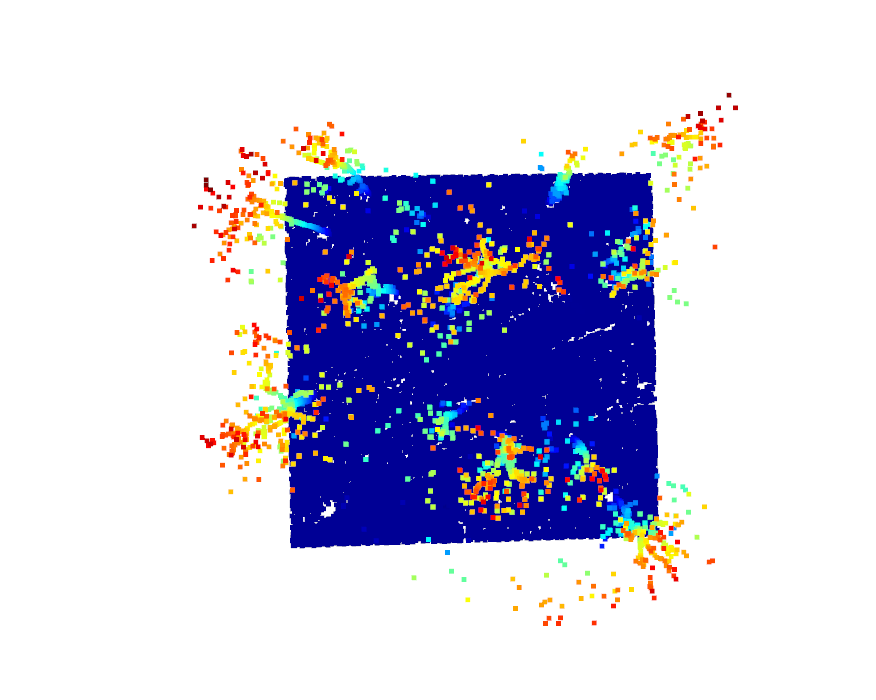
\includegraphics[height=6cm]{imaxes/slice_sup.png}
  \caption{Nube de puntos Original desde arriba}
  \label{fig:slice_top}
\end{subfigure}
\begin{subfigure}[t]{.4\textwidth}
  \centering
  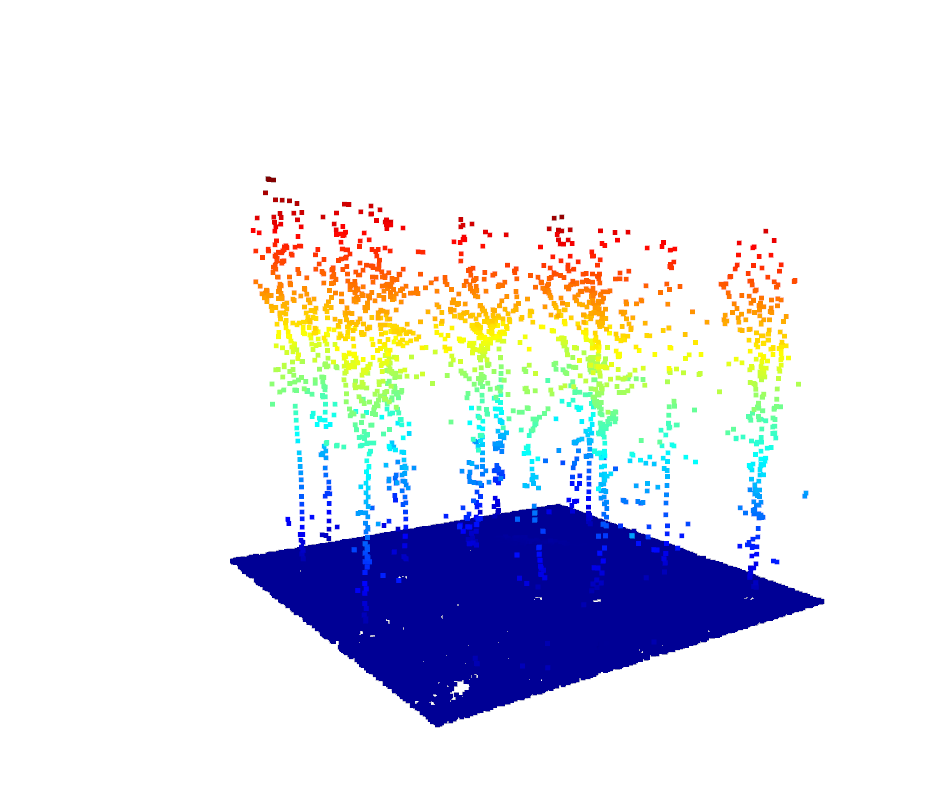
\includegraphics[height=6cm]{imaxes/slice_lat.png}
  \caption{Nube de puntos Original vista lateral}
  \label{fig:slice_lat}
\end{subfigure}
\begin{subfigure}[t]{.4\textwidth}
  \centering
  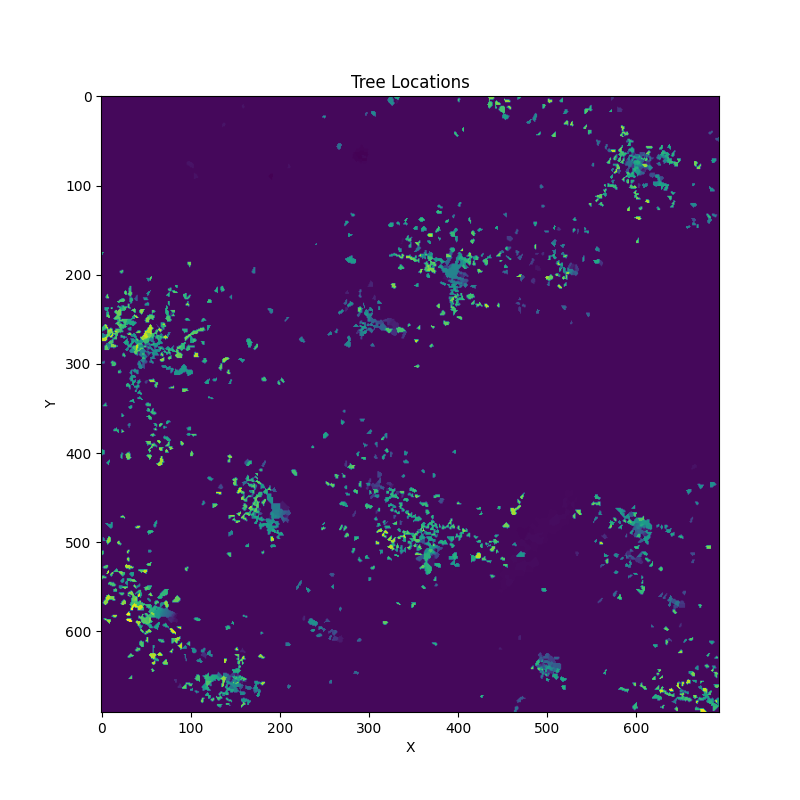
\includegraphics[height=6cm]{imaxes/chm.png}
  \caption{Mapa de alturas}
  \label{fig:chm}
\end{subfigure}%
\begin{subfigure}[t]{.4\textwidth}
  \centering
  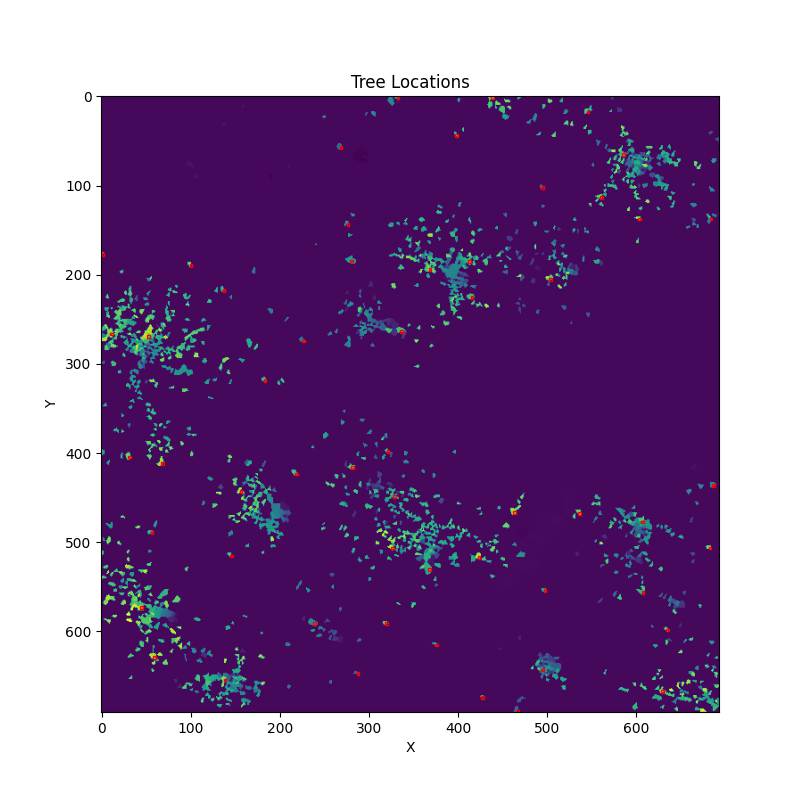
\includegraphics[height=6cm]{imaxes/chm_with_trees.png}
  \caption{Mapa de alturas con los Maximos}
  \label{fig:chm_max}
\end{subfigure}

\caption{Ejemplo de Obtencion de arboles mediante maximos}
\label{fig:chmexample}
\end{figure}

\subsection{Detección de árboles mediante árboles}

Una vez obtenidos los puntos con potencial de ser árboles, obtendremos una sección cilíndrica de puntos con centro en ese punto. Esta sección tiene un radio que determinaremos, y dentro de ella se tienen que encontrar los puntos que conforman ese \textit{árbol}.

Los troncos de los árboles tienden a tener una estructura que forma una línea, aunque en ciertas especies, llegada cierta altura, comienza a tener muchas ramificaciones; hasta ese punto forma una línea.

Lo que buscamos es ser capaces de encontrar esa linealidad en esa sección. Para eso, la partiremos en \textit{slices} de la misma altura y obtendremos el centroide. Las slices tendrán un tamaño fijo que definimos previamente. Un centroide representa el centro geométrico de los puntos de esa rodaja. Con una lista de estos, obtendremos un score en función de que también se ajuste a una línea, y en función de si es mayor a un umbral o no, se determinará si es realmente un árbol.


Para obtener este valor de que tan bien se ajustan a una linea usaremos el método de los mínimos cuadrados. Este método busca minimizar la suma de los cuadrados de las diferentes ordenadas. La ecuación de una línea en 3D se representa como $z = ax + by + c$, donde $z$ es la coordenada vertical y $x$ e $y$ son las coordenadas horizontales. Los coeficientes $a$, $b$, y $c$ se determinan para minimizar la función de error:

\[
E(a, b, c) = \sum_{i=1}^{n} (z_i - (ax_i + by_i + c))^2
\]

donde $n$ es el número de puntos y $(x_i, y_i, z_i)$ son las coordenadas de cada punto. La optimización se realiza para encontrar los valores de $a$, $b$, y $c$ que minimizan esta función, lo que permite construir la ecuación de la línea que mejor se ajusta a los datos.

Si nuestro algoritmo solo tuviera en cuenta eso podrían surgir problemas al encontrarse con ramificaciones o con puntos que aun que estén dentro del cilindro pueden ser de otro árbol o ruido. 
Con el fin de hacer el algoritmo más robusto, antes de calcular el centroide de cada slice, se aplica un algoritmo al conjunto de puntos que la conforman y se aplica un algoritmo de \textit{clustering}, en nuestro caso usamos DBSCAN, que se basa en la agrupación en la densidad de puntos en una zona. En una primera implementación, en el caso de tener más de un centroide en una slice podríamos seleccionar solo el que se ajuste mejor a una recta con los centroides previos, pero con esta decisión estaríamos descartando centroides que aunque en el contexto de esa sección se ajustan peor, en el contexto de todo el árbol pueden tener un mejor ajuste.

\begin{figure}[h]
\centering
    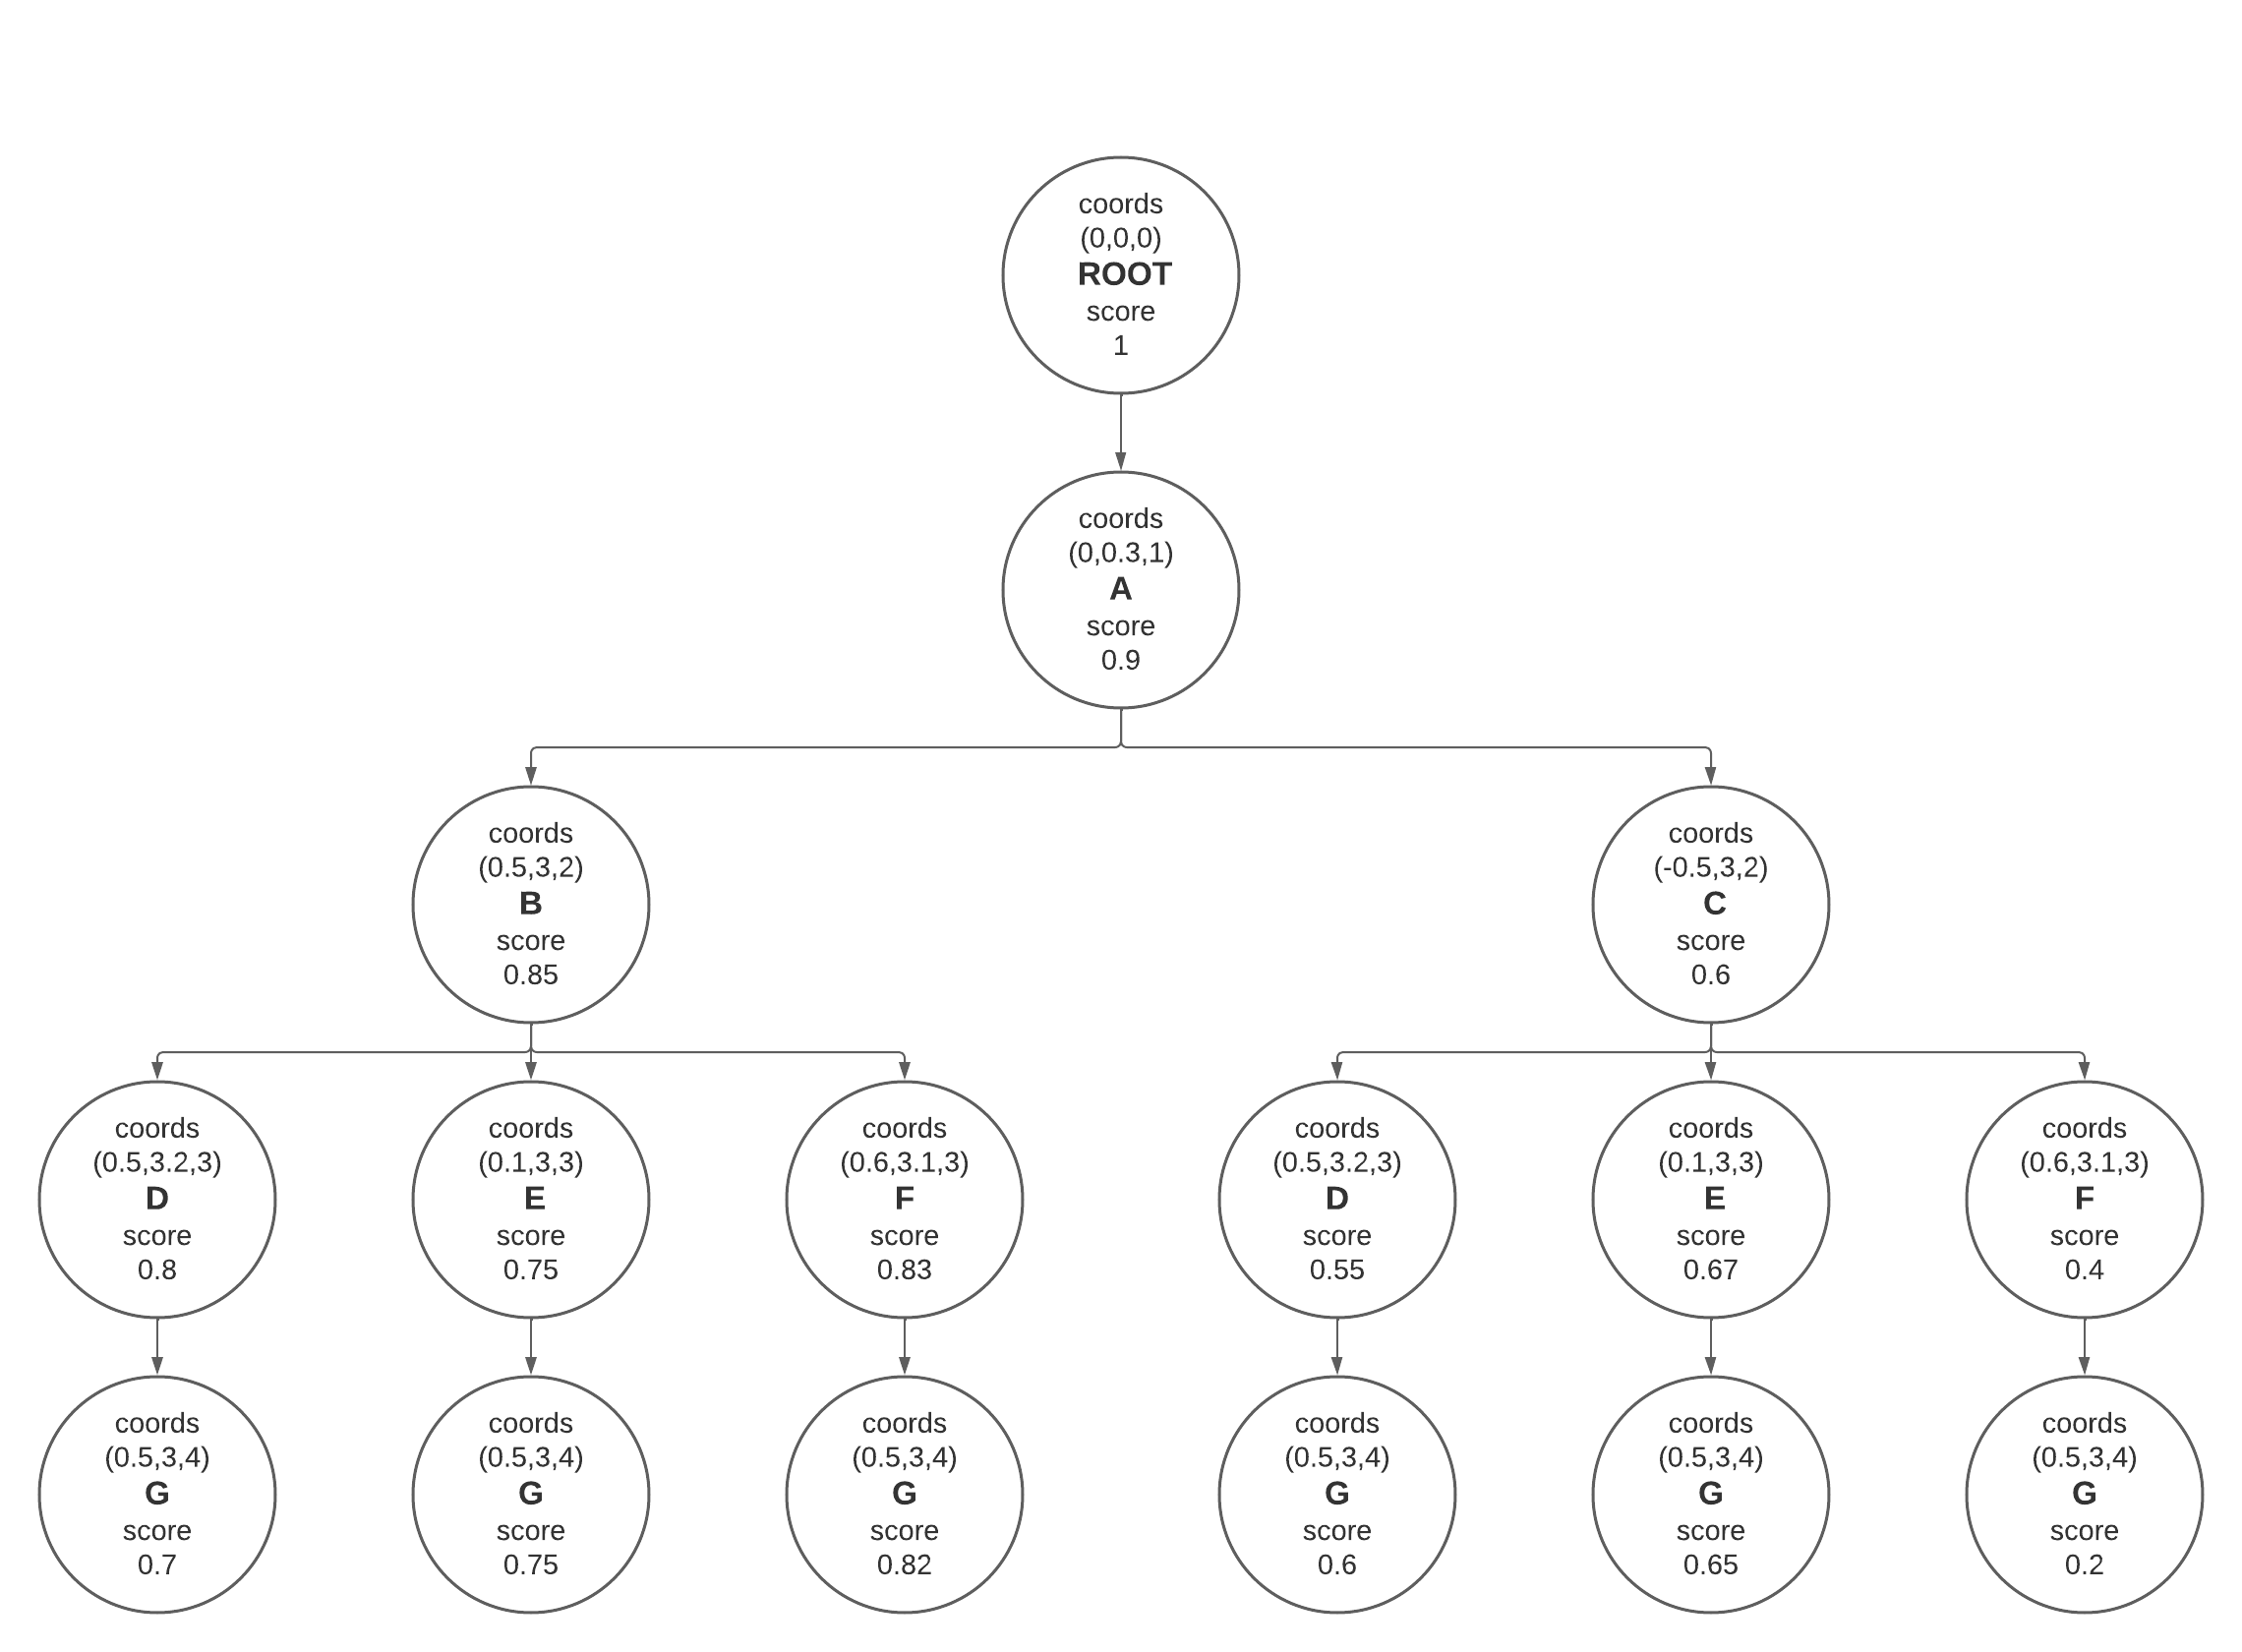
\includegraphics[width=13cm]{imaxes/Diagrama_arb.png}
    \caption{Ejemplo de un árbol de centroides}
    \label{fig:diagFlujoarb}
\end{figure}


Por lo que para evitar esto se guardan todos en una estructura de árbol que contiene las coordenadas del centroide y el ajuste a una linea con el resto de centroides, a cada nodo se le añaden los slices del siguiente slice. 
En la figura \ref{fig:diagFlujoarb} vemos como sería uno de estos árboles. Al tener el árbol lo que haremos será mirar los nodos hoja y mirar cuál es el que tiene mayor score, es decir, que mejor se ajuste a una línea y a partir de ese nodo iremos recorriendo la estructura de datos asta la raíz para obtener todos los centroides por los que pasa.

Para terminar mostraremos el código que realiza esta parte y lo comentaremos en relación al algoritmos explicado. Lo primero que hacemos para cada puntos es obtener la sección cilíndrica con el radio que definimos. A continuación para evitar detectar arbustos o maleza comprobamos si en ese cilindro hay un mínimo de puntos, este es un parámetro constante definido como constante.


Si tiene mas de el mínimo de puntos se procede a llamar a la función que divide ese cilindro en diferentes secciones y obtiene los centroides mediante el algoritmo que mencionamos antes. Una vez con los centroides volvemos a calcular el ajuste de los puntos y mediante un umbral decidimos si ese punto es realmente un árbol o no.

Ahora con la figura \ref{fig:ejemplotree} veremos un ejemplo de como seria el proceso para la obtención de los centroides. La figura \ref{fig:tree} es la nube de puntos de la sección tubular, en este ejemplo vemos claramente el tronco. A continuación en \ref{fig:tree_sliced} se ejemplifica como dividimos esa nube de puntos en 7 slices, para cada uno obtendremos los centroides y después de entre todos escogeremos los que mejor forme una linea \ref{fig:tree_sliced_centroids} y \ref{fig:tree_sliced_res}.




\begin{lstlisting}[language=Python, caption={Código para la busqueda de máximos }, label=lst:detectT]
def detect_trees(point_cloud, query_coords, radius_threshold):
    # create a list to save the locations of the trees that are tubular
    tubular_tree_locations = []
    no_tubular_tree_locations = []

    for query_coord in query_coords:

        distances = np.linalg.norm(point_cloud[:, :2] - query_coord[:2], axis=1)
        filtered_indices = np.where(distances <= radius_threshold)[0]
        filtered_points = point_cloud[filtered_indices]
        
        if len(filtered_points) < min_tree_samples:
            continue
        else:
            pcd = o3d.geometry.PointCloud()
            pcd.points = o3d.utility.Vector3dVector(filtered_points)
            
            centroids = slice_and_get_points_tree(filtered_points, slice_height)
            centroids = np.array(centroids)

            if len(centroids) > 4 and not np.isnan(centroids).any():

                r2 = calculate_r_squared(centroids)
                is_line = r2 > r_squared_threshold

                if is_line:
                    tubular_tree_locations.append(query_coord)
                else:
                    no_tubular_tree_locations.append(query_coord)
    return tubular_tree_locations
\end{lstlisting}

\begin{figure}[h]
  \begin{subfigure}{0.5\textwidth}
    \centering
    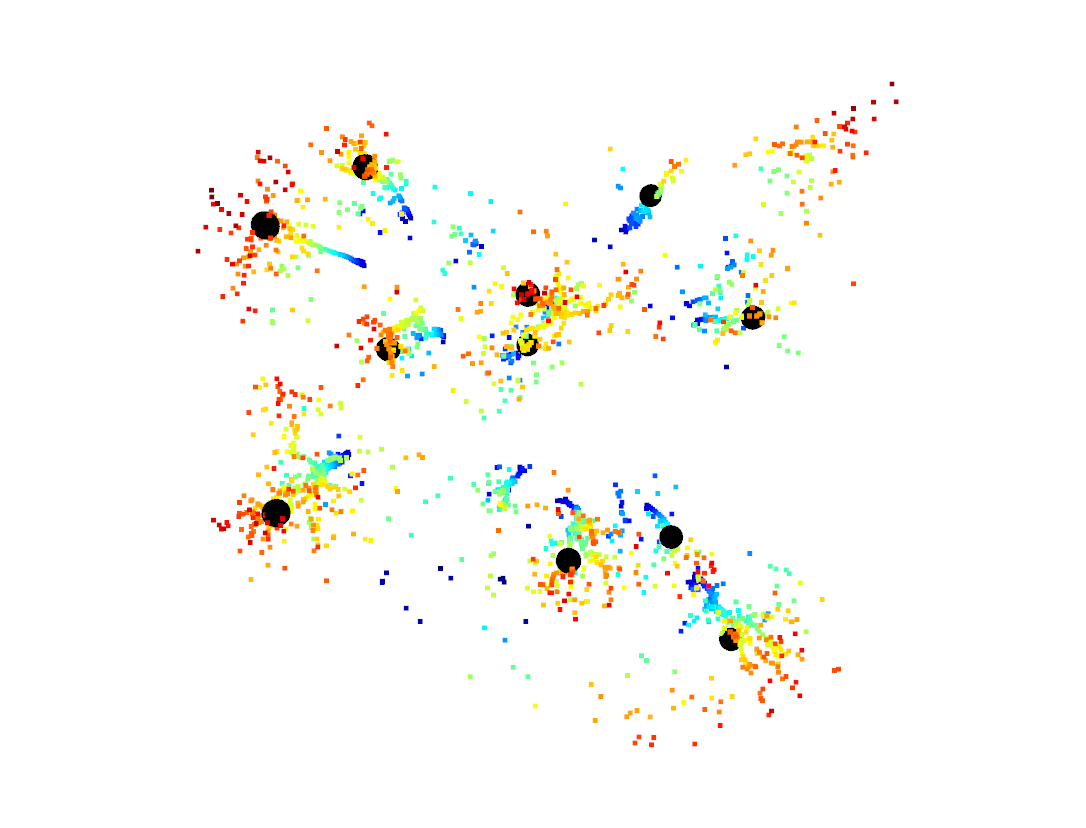
\includegraphics[width=0.8\linewidth]{imaxes/detecsup.png}
    \caption{Puntos detectamos arboles vista superior}
    \label{fig:last1}
  \end{subfigure}%
  \begin{subfigure}{0.5\textwidth}
    \centering
    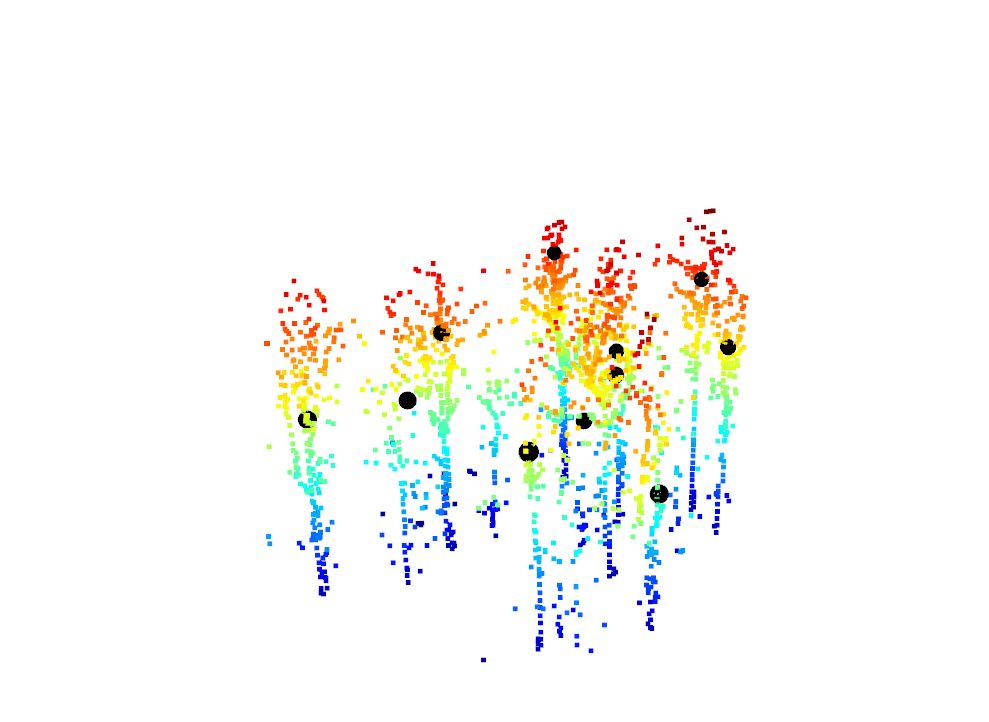
\includegraphics[width=0.8\linewidth]{imaxes/deteclat.png}
    \caption{Puntos detectamos arboles vista lateral}
    \label{fig:last}
  \end{subfigure}
  \caption{Ejemplo de puntos detectados como arboles, puntos negros son un árbol}
  \label{fig:algo2}
\end{figure}

\begin{figure}
\centering
\begin{subfigure}[t]{.5\textwidth}
  \centering
  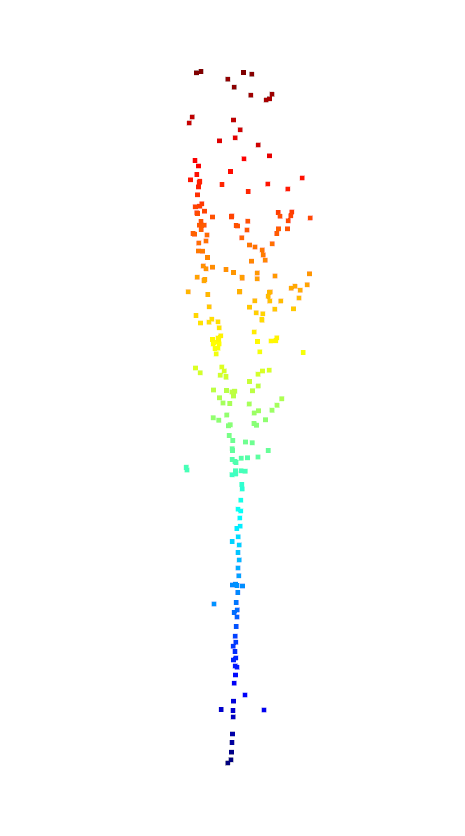
\includegraphics[height=5cm]{imaxes/tree.png}
  \caption{Nube de puntos del árbol}
  \label{fig:tree}
\end{subfigure}%
\begin{subfigure}[t]{.5\textwidth}
  \centering
  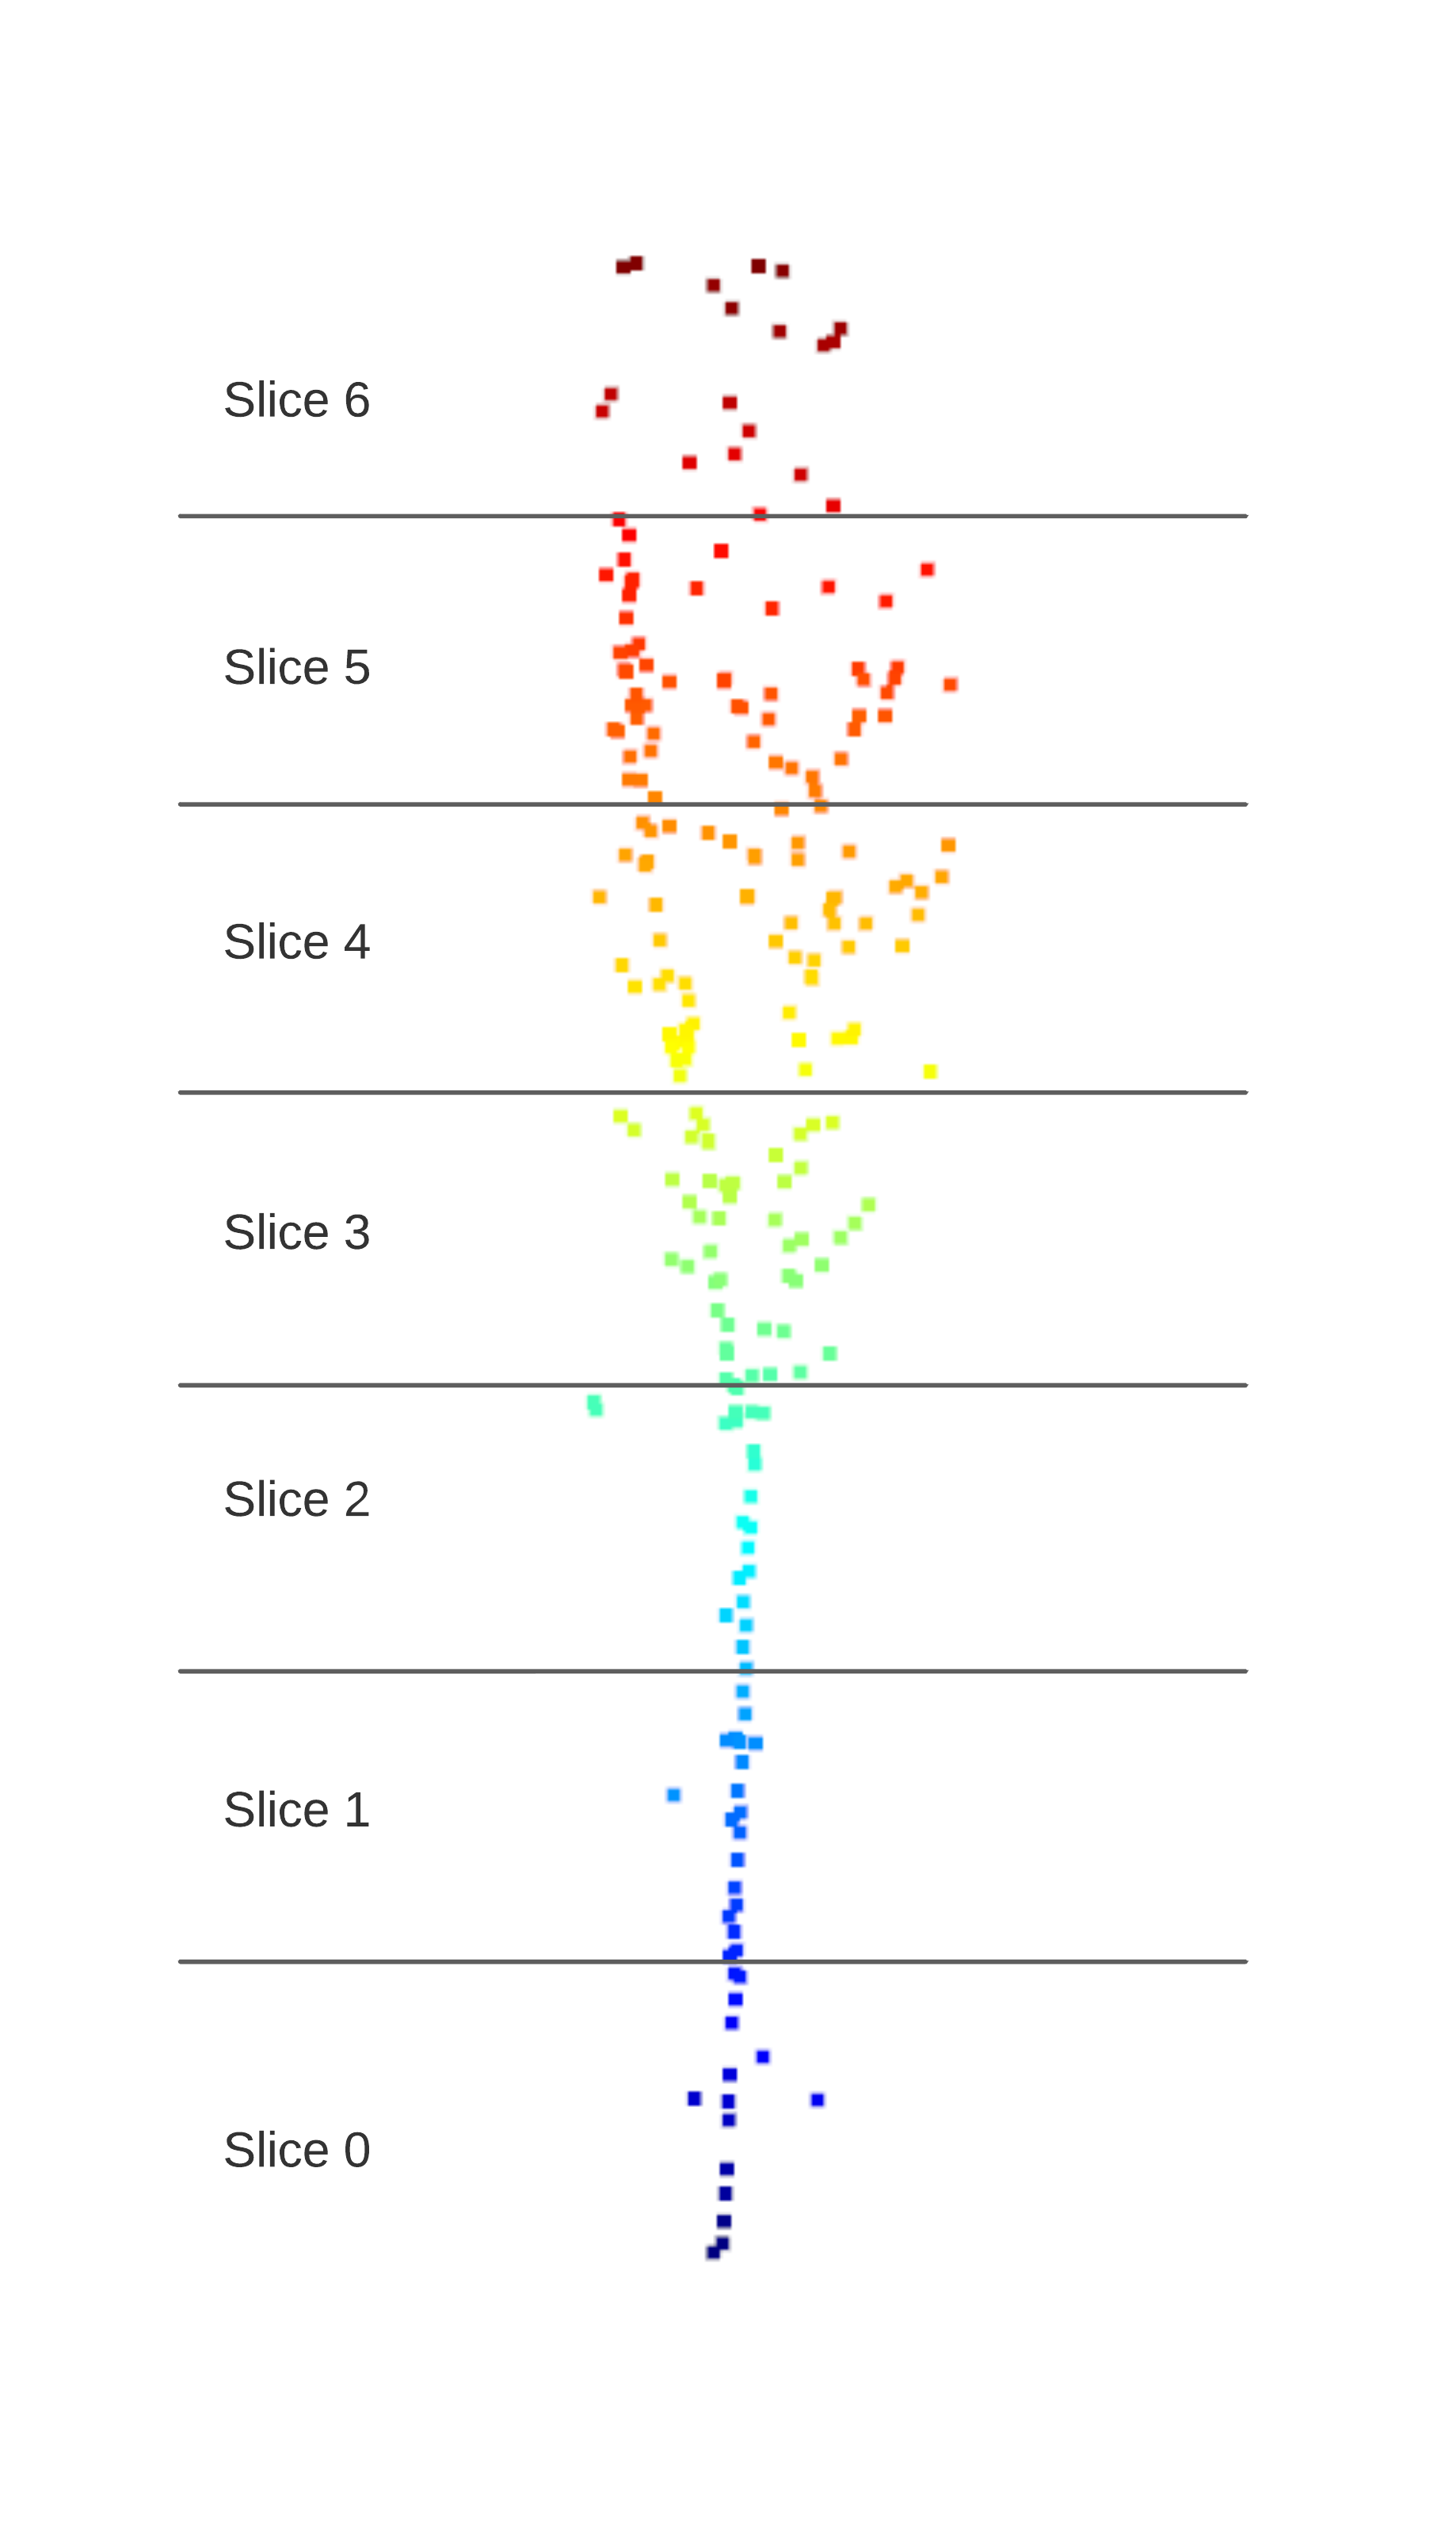
\includegraphics[height=5cm]{imaxes/tree_slices.png}
  \caption{Árbol dividida en 7 slices}
  \label{fig:tree_sliced}
\end{subfigure}

\begin{subfigure}[t]{.5\textwidth}
  \centering
  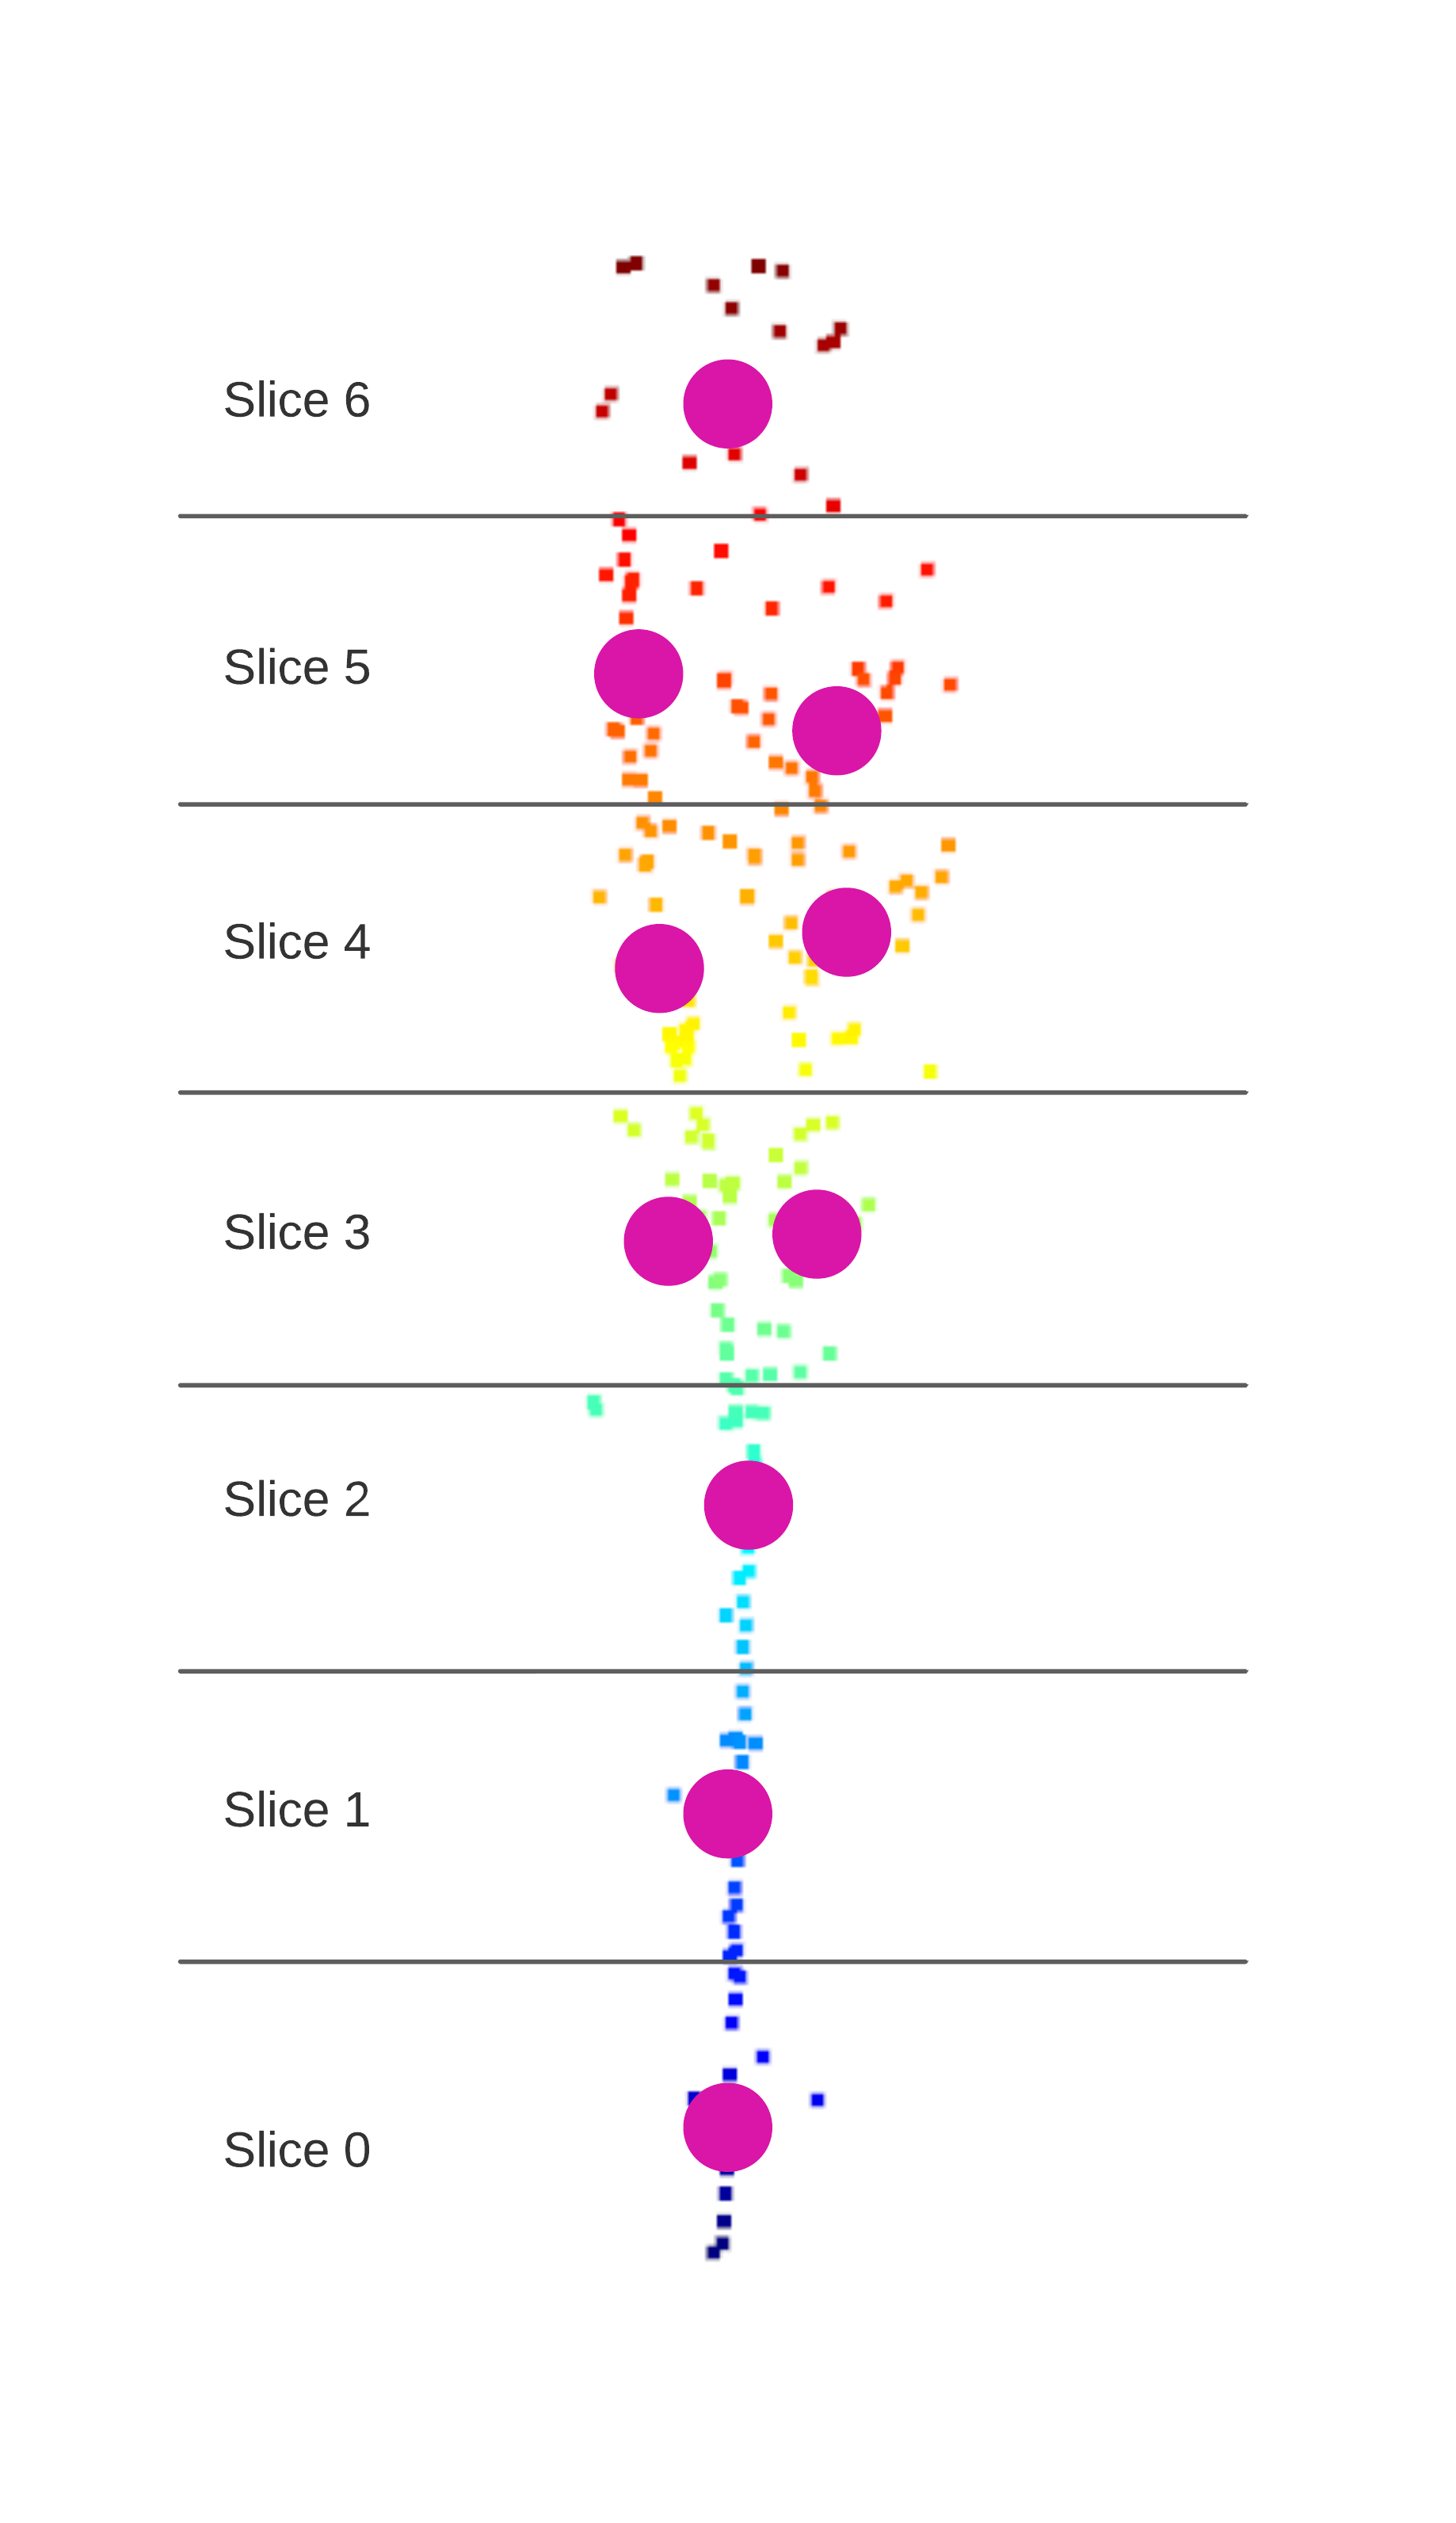
\includegraphics[height=5cm]{imaxes/tree_slices_centroids.png}
  \caption{Árbol con los centroides }
  \label{fig:tree_sliced_centroids}
\end{subfigure}%
\begin{subfigure}[t]{.5\textwidth}
  \centering
  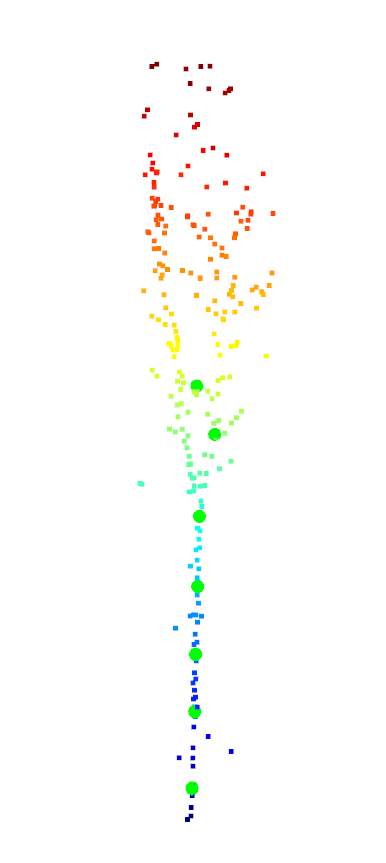
\includegraphics[height=5cm]{imaxes/tree_centroides.png}
  \caption{Árbol con centroides ajustados}
  \label{fig:tree_sliced_res}
\end{subfigure}

\caption{Ejemplo del proceso de obtención de los slices}
\label{fig:ejemplotree}
\end{figure}




